\documentclass[]{article}
\usepackage{geometry}   % my added package "geometry"
\geometry{letterpaper,tmargin=1in,bmargin=1in,lmargin=2.2cm,rmargin=2.2cm}
\usepackage[colorlinks,bookmarksopen,bookmarksnumbered,
citecolor=green,urlcolor=red]{hyperref}
\hypersetup{pdfauthor={Name}}
%%%%%%%%%%%%%%%%%%%%%%%%%%%%%%%%%%%%%%%%%%%%%%%%%%%%%%%%%%%%%%%%%%%%%%%%%
%\usepackage{graphicx}
\usepackage{graphics}
\usepackage{epsfig}
\usepackage{epstopdf}
\usepackage{amsfonts}
\usepackage{amssymb}
\usepackage{booktabs}
\usepackage{color,soul}
%%%%%%%%%%%%%%%%%%%%%%%%%%%%%%%%%%%%%%%%%%%%%%%%%%%%%%%%%%%%%%%%%
\usepackage{amsmath}
\usepackage{cleveref}
%\usepackage[fleqn]{amsmath}
\usepackage{lineno}
\usepackage{tikz}
\usepackage{standalone}
\usetikzlibrary{calc,patterns,arrows.meta,shapes.arrows,intersections,positioning}
\usetikzlibrary{decorations.pathmorphing,backgrounds,fit,petri}
\usepackage[percent]{overpic}
%%%%%%%%%%%%%%%%%%%%%%%%%%%%%%%%%%%%%%%%%%%%%%%%%%%%%%%%%%%%%%%%%
\usepackage{xcolor}
\usepackage{listings}
\lstset { %
	language=C++,
	backgroundcolor=\color{black!5}, % set backgroundcolor
	basicstyle=\footnotesize,% basic font setting
}
%%%%%%%%%%%%%%%%%%%%%%%%%%%%%%%%%%%%%%%%%%%%%%%%%%%%%%%%%%%%%%%%%
\renewcommand\thesubsection{\thesection\Alph{subsection}}
%%%%%%%%%%%%%%%%%%%%%%%%%%%%%%%%%%%%%%%%%%%%%%%%%%%%%%%%%%%%%%%%%
%opening
\begin{document}
\title{HiperLife Tutorial: Poisson Equation}
\author{LaCàN}
\maketitle

\linenumbers
\section{Introduction} \label{sec: Int}
\subsubsection{Problem Definition} \label{sec: pd} 
Poisson Equation is a simple elliptic model, given by
\begin{equation}\label{eq1}
	\begin{aligned}
		 -\Delta U = -\nabla^2 U = -\frac{\partial^2 U}{\partial x_{1}^2} - 
		\frac{\partial^2 U}{\partial x_{2}^2}=f
	\end{aligned}
\end{equation}
We will use this equation in this example for introducing the implemention of finite
element method in the HiperLife. Notice that here we have used $f = 0$.
\subsubsection{Boundary Condition} \label{sec: B.C}
As shown in Fig 1, We have used homogeneous Dirichlet ($U=0 ,\quad U=1$) along the lines ($x_{1}=0,\quad x_{1}=1$), and along the lines ($x_{2}=0.5,\quad x_{2}=1$) we applied Inhomogenous Dirichelet ($U=x_{1} ,\quad U=x_{1}^2$), respectively.

\begin{figure}[htbp]
	\centering
	
\documentclass[preprint,12pt,a4]{standalone}
\usepackage{geometry}   % my added package "geometry"
\geometry{letterpaper,tmargin=1in,bmargin=1in,lmargin=2.5cm,rmargin=2.5cm}
\usepackage{tikz}
\usetikzlibrary{calc,patterns,arrows.meta,shapes.arrows,intersections,positioning}
\usetikzlibrary{decorations.pathmorphing,backgrounds,fit,petri}
\usepackage{standalone}
\begin{document}
	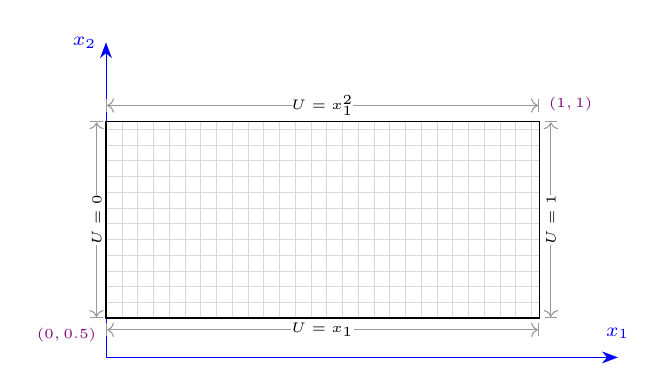
\begin{tikzpicture} [{place/.style={rectangle,draw=blue!50,fill=blue!20,ultra thin,inner sep=0.8mm}},{place2/.style={circle,draw=black!50,ultra thin,inner sep=0.8mm}},{linest/.style={color=gray,ultra thin}}]
	%%coordinates of corners of Beam
	\coordinate (A) at (0.0,0.0);
	\coordinate (B) at (5.5,0.0);
	\coordinate (D) at ($(A)+(0.0,2.5)$);
	\coordinate (C) at ($(B)+(D)$);
	%%axes
	\draw [{Stealth[length=2mm]}-{Stealth[length=2mm]}, help lines,blue] ($(B)+(1,-0.5)$) -- (0,-0.5) -- ($(D)+(0,1)$);
	\node [below,color = blue,font=\scriptsize] at ($(B)+(1,0)$) {$x_1$};
	\node [left,color = blue,font=\scriptsize] at ($(D)+(0,1)$) {$x_2$};
	%%fixed boundary
	%\draw [pattern = crosshatch] ($(A)-(0.1,0.3)$) rectangle ($(D)+(0.0,0.3)$);
	%%mesh
	\draw [line width=0.1pt,gray!30,step=2mm](A) grid (C);
	%%Beam	
	\draw [color=black](A)node[font=\tiny, violet,below left]{$(0,0.5)$} -- (B) -- (C) node[font=\tiny, violet,above right]{$(1,1)$} -- (D) -- cycle;
	%%Concentrate Force Vector
	%\draw [-{Latex[length=2mm]},color=purple, thick] ($(C)+(0.0,1.0)$) -- (C);
	%\node[above,color=purple] at ($(C)+(0.0,1.0)$) {$P$};
	%%B.C
	\draw [|<->|,gray!80]($(A)+(0,-0.15)$) --($(B)+(0,-0.15)$) node[fill=white,midway,inner sep=0.1pt, font=\tiny,text=black] {$U=x_{1}$};
	\draw [|<->|,gray!80]($(B)+(0.15,0.0)$)--($(C)+(0.15,0.0)$) node [fill=white,midway, sloped, font=\tiny, inner sep=0.05pt, text=black] {$U=1$};
	
	\draw [|<->|,gray!80]($(C)+(0,0.2)$) --($(D)+(0,0.2)$) node[fill=white,midway,inner sep=0.01pt, font=\tiny,text=black] {$U=x_{1}^2$};
	\draw [|<->|,gray!80]($(A)+(-0.12,0.0)$)--($(D)+(-0.12,0.0)$) node [fill=white,midway,sloped, font=\tiny, inner sep=0.05pt, text=black] {$U=0$};
	\end{tikzpicture}
\end{document}
	\caption{Schematic of Geometry in $\Omega =[0,1]\times[0.5,1]$ and Boundary conditions on $\partial \Omega$.}
	\label{fig_SB}
\end{figure}

\section{Formulation} \label{sec: frml}
\subsubsection{Weak Form} \label{sec: WF}
To establish the weak form of Eq. \ref{eq1}, it is multiplied with a weight-function, $w(x, y)$ to obtain
\begin{equation}\label{eq2}
	\begin{aligned}[b]
		-w\nabla^2 U = wf
	\end{aligned}
\end{equation}
By integrating this expression over $\Omega$, we have

\begin{equation}\label{eq3}
	\begin{aligned}[b]
		-\int_\Omega w\nabla^2 U = \int_\Omega wf
	\end{aligned}
\end{equation}
We know from calculus that $\nabla(w\nabla U) = \nabla w \cdot \nabla U + w\nabla ^2 U$. So we can write
\begin{equation}\label{eq4}
	\begin{aligned}[b]
		-\int_\Omega w\nabla^2U = \int_{\Omega} \nabla(w\nabla U) - \int_{\Omega} \nabla w \cdot \nabla U = \int_\Omega wf dA
	\end{aligned}
\end{equation}
Using Gauss’s theorem we get
\begin{equation}\label{eq5}
	\begin{aligned}[b]
		\int_\Omega \nabla(w\nabla U) = \int_{\partial\Omega} w \nabla U \cdot n dS = 0
	\end{aligned}
\end{equation}
Eq. \ref{eq4} now reduces to
\begin{equation}\label{eq6}
	\begin{aligned}[b]
		\int_\Omega w\nabla^2U = - \int_{\Omega} \nabla w \cdot \nabla U
	\end{aligned}
\end{equation}
so we get 
\begin{equation}\label{eq7}
	\begin{aligned}[b]
		\int_{\Omega} \nabla w \cdot \nabla U dA = \int_\Omega wf dA
	\end{aligned}
\end{equation}
\subsubsection{Basis Function} \label{sec: Basis Func}
We need to define basis functions for our 2D-domain and by it we can give an approximation of U.
\begin{equation}\label{eq8}
	\begin{aligned}[b]
		U(x,y) =\sum_{i=1}^{n} u_{i}\phi_{i}(x_{1},x_{2})
	\end{aligned}
\end{equation}
by applying Gelerkin method the weight function is the same as basis function.
\begin{equation}\label{eq9}
	\begin{aligned}[b]
		w_{i} =\phi_{i}
	\end{aligned}
\end{equation}
in isoparametric concept even geometry is interpolated by same function. so
\begin{equation}\label{eq10}
	\begin{aligned}[b]
		X(x_{1},x_{2}) =\sum_{i=1}^{n} x_{i}\phi_{i}(x_{1},x_{2})
	\end{aligned}
\end{equation}
\subsubsection{Element} \label{sec: elem}
Quadrilateral Elements is the simplest quadrilateral element consists of
four nodes. The associated interpolation functions for geometry and field
variables are bilinear. Let $\phi_{I}=N_I $ at element $T$.
\begin{equation}\label{eq11}
	\begin{aligned}[b]
		N_{I}(\xi, \eta) = \frac{1}{4}(1+\xi_I\xi)(1+\eta_I\eta)
	\end{aligned}
\end{equation}
where $\xi_{I}$ and $\eta_{I}$ are the corner coordinates at element $T$ in domain of $\Omega_{T} \in (-1,1)^2$.

\begin{figure}[htbp]
	\centering
	\documentclass[preprint,12pt,a4]{standalone}
\usepackage{geometry}   % my added package "geometry"
\geometry{letterpaper,tmargin=1in,bmargin=1in,lmargin=2.5cm,rmargin=2.5cm}
\usepackage{tikz}
\usetikzlibrary{calc,patterns,arrows.meta,shapes.arrows,intersections,positioning}
\usetikzlibrary{decorations.pathmorphing,backgrounds,fit,petri}
\usepackage{standalone}
%
\begin{document}
	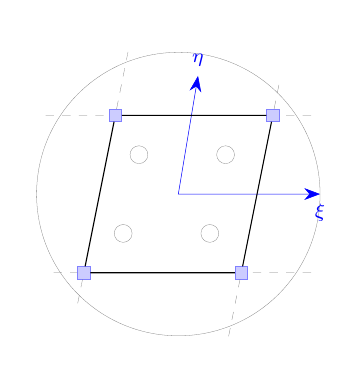
\begin{tikzpicture} [{place/.style={rectangle,draw=blue!50,fill=blue!20,ultra thin,inner sep=0.8mm}},{place2/.style={circle,draw=black!50,ultra thin,inner sep=0.8mm}},{linest/.style={color=gray,ultra thin}}]
		%%circle
		\draw [linest,fill=white](5.2,3.5) circle [radius=18mm];
		%axes
		\draw [{Stealth[length=2mm]}-{Stealth[length=2mm]}, help lines,blue] (7,3.5)node[below,font=\scriptsize]{$\xi$} -- (5.2,3.5) -- (5.45,5)node[above,font=\scriptsize] {$\eta$};
		%%element Nodes
		\node at (4.0,2.5) [place] (1) {};
		%\node at (5.0,2.5) [place] (2) {};
		\node at (6.0,2.5) [place] (3) {};
		%\node at (4.2,3.5) [place] (4) {};
		%\node at (5.2,3.5) [place] (5) {};
		%\node at (6.2,3.5) [place] (6) {};
		\node at (4.4,4.5) [place] (7) {};
		%\node at (5.4,4.5) [place] (8) {};
		\node at (6.4,4.5) [place] (9) {};
		
		\node at (4.5,3.0) [place2] {};
		\node at (5.6,3.0) [place2] {};
		\node at (4.7,4.0) [place2] {};
		\node at (5.8,4.0) [place2] {};
		\node at (3.5,2.5) [place2, draw = none] (10) {};
		\node at (7.0,2.5) [place2, draw = none] (11) {};
		\node at (3.4,4.5) [place2, draw = none] (12) {};
		\node at (7.0,4.5) [place2, draw = none] (13) {};
		\node at (3.9,2.0) [place2, draw = none] (14) {};
		\node at (5.8,1.5) [place2, draw = none] (15) {};
		\node at (4.6,5.5) [place2, draw = none] (16) {};
		\node at (6.5,5.0) [place2, draw = none] (17) {};
		%%element border
		\draw [-] (1) --(3)--(9)--(7)--(1);
		\draw [dashed,linest] (10) -- (1)--(14);
		\draw [dashed,linest] (11) -- (3)--(15);
		\draw [dashed,linest] (12) -- (7)--(16);
		\draw [dashed,linest] (13) -- (9)--(17);
	\end{tikzpicture}
\end{document}
	\caption{Schematic of an Element.}
	\label{fig_el}
\end{figure}
%
In this example each node only have one degree of freedom and for the purpose of discretization we use $500 \times 500$ uniform mesh.
\subsubsection{Elemental Integral} \label{sec: elem int}
  We want to compute the integral at Eq. \ref{eq7} over the element $T$
\begin{equation}\label{eq12}
	\begin{aligned}[b]
		\int_{\Omega_{T}} (\frac{\partial N}{\partial x_{1}}
		\frac{\partial N}{\partial x_{1}}+\frac{\partial N}{\partial x_{2}} 
		\frac{\partial N}{\partial x_{2}})U dA = \int_{\Omega_{T}} Nf dA
	\end{aligned}
\end{equation}
by the linear mapping between $(\xi,\eta)$ and $(x_{1},x_2)$, we can define $\frac{\partial N}{\partial x_{1}}$ and $\frac{\partial N}{\partial x_{2}}$
\begin{equation}\label{eq13}
	\begin{aligned}[b]
&
		\frac{\partial N}{\partial \xi} = \frac{\partial N}{\partial x_{1}}\frac{\partial x_{1}}{\partial \xi}+\frac{\partial N}{\partial x_{2}}\frac{\partial x_{2}}{\partial \eta}\\
& 
		\frac{\partial N}{\partial \eta} = \frac{\partial N}{\partial x_{1}}\frac{\partial x_{1}}{\partial \xi}+\frac{\partial N}{\partial x_{2}}\frac{\partial x_{2}}{\partial \eta}
	\end{aligned}
\end{equation}
Since $x=x(\xi,\eta)$, we get

\begin{equation}\label{eq14}
	\begin{aligned}[b]
		\begin{bmatrix}
			dx_{1}\\
			\\
			dx_{2}  
		\end{bmatrix}
		= \begin{bmatrix}
			\frac{\partial x_{1}}{\partial \xi}       & \frac{\partial x_{2}}{\partial \xi} \\
			\\
			\frac{\partial x_{1}}{\partial \eta}       &\frac{\partial x_{2}}{\partial \eta}\\
		\end{bmatrix}
		\begin{bmatrix}
			d \xi\\
			\\
			d \eta
		\end{bmatrix}
	\end{aligned}
\end{equation}
%
by defining Jacobian as
\begin{equation}\label{eq15}
	\begin{aligned}[b]
		J = \begin{bmatrix}
			\frac{\partial x_{1}}{\partial \xi}       & \frac{\partial x_{2}}{\partial \xi} \\
			\\
			\frac{\partial x_{1}}{\partial \eta}       &\frac{\partial x_{2}}{\partial \eta}\\
			\end{bmatrix}
	\end{aligned}
\end{equation}
so we can rewrite the Eq. \ref{eq13}

\begin{equation}\label{eq16}
	\begin{aligned}[b]
\begin{bmatrix}
	\frac{\partial N}{\partial x_{1}}\\
	\\
	\frac{\partial N}{\partial x_{2}}  
\end{bmatrix}
= J^{-1}
\begin{bmatrix}
	\frac{\partial N}{\partial \xi}\\
	\\
	\frac{\partial N}{\partial \eta}
\end{bmatrix}
	\end{aligned}
\end{equation}
 by obtaining the terms Eq \ref{eq12} now we can calculate the integral. So the elements of tangent matrix $K$ could be defined as
\begin{equation}\label{eq17}
	\begin{aligned}[b]
		K(i,j) = \int_{\Omega_{T}} (\frac{\partial N_{i}}{\partial x_{1}}
		\frac{\partial N_{j}}{\partial x_{1}}+\frac{\partial N_{i}}{\partial x_{2}} 
		\frac{\partial N_{j}}{\partial x_{2}}) dA
	\end{aligned}
\end{equation}
and for external source 
\begin{equation}\label{eq18}
	\begin{aligned}[b]
		F(i) = \int_{\Omega_{T}} N_{i}f dA
	\end{aligned}
\end{equation}
keep in mind that in our case $f=0$. Note that $dA=dx_{1} \times dx_{2}=jd\xi d\eta$, which $j=det(J)$.
\begin{figure}[htbp]
	\centering
	\documentclass[preprint,12pt,a4]{standalone}
\usepackage{geometry}   % my added package "geometry"
\geometry{letterpaper,tmargin=1in,bmargin=1in,lmargin=2.5cm,rmargin=2.5cm}
\usepackage{tikz}
\usetikzlibrary{calc,patterns,arrows.meta,shapes.arrows,intersections,positioning}
\usetikzlibrary{decorations.pathmorphing,backgrounds,fit,petri}
\usepackage{standalone}
%
\begin{document}
	\begin{tikzpicture} [{place/.style={rectangle,draw=blue!50,fill=blue!20,ultra thin,inner sep=0.8mm}},{place2/.style={circle,draw=black!50,ultra thin,inner sep=0.8mm}},{linest/.style={color=gray,ultra thin}}]
		%axes
		\draw [{Stealth[length=2mm]}-{Stealth[length=2mm]}, help lines,blue] (5.0,0)node[above,font=\scriptsize]{$\xi$} -- (0.0,0.0) -- (0.0,5.0)node[right,font=\scriptsize] {$\eta$};
		%%element Nodes
		\node at (0.0,0.0) [place,fill=white] (1) {};
		\node at (4.0,0.0) [place,fill=white] (2) {};
		\node at (4.0,4.0) [place,fill=white] (3) {};
		\node at (0.0,4.0) [place,fill=white] (4) {};
		
		\node at (1.0,1.0) [place2,fill=black!60] {};
		\node at (3.0,1.0) [place2,fill=black!60] {};
		\node at (1.0,3.0) [place2,fill=black!60] {};
		\node at (3.0,3.0) [place2,fill=black!60] {};
		%%element border
		\draw [-] (1) -- (2) -- (3) -- (4) --(1);
	\end{tikzpicture}
\end{document}
	\caption{2D integration on Quadrilateral Element.}
	\label{fig_int}
\end{figure} 
\subsubsection{Integration method} \label{sec: int}
Let $f(\xi_{i},\eta_{i})=j(\frac{\partial N_{i}}{\partial x_{1}}
\frac{\partial N_{j}}{\partial x_{1}}+\frac{\partial N_{i}}{\partial x_{2}} 
\frac{\partial N_{j}}{\partial x_{2}})$, then by Gauss–Legendre quadrature we have
\begin{equation}\label{eq19}
	\begin{aligned}[b]
		\int_{-1}^1 \int_{-1}^1 f(\xi_{i},\eta_{i}) d\xi d\eta = \sum_{k=1}^{n}\sum_{l=1}^{m} \omega_{k}\omega_{l}f(\hat{\xi_{i}},\hat{\eta_{i}})
	\end{aligned}
\end{equation}
where $n$ and $m$ are the number of integration points used in each direction, $\omega$ is quadrature weights, $\hat{\xi_{i}}$ and $\hat{\eta_{i}}$ are the roots of the $n$th Legendre polynomial. In this example we use $2 \times 2$ integration as it shown in Fig. \ref{fig_int}. Which the value of  quadrature weights are the same $\omega_{p}=1$, and coordinate of guass points would be:  $(\xi_{p}, \eta_{p})=\{(-\frac{1}{\sqrt{3}},-\frac{1}{\sqrt{3}}),  (\frac{1}{\sqrt{3}}, -\frac{1}{\sqrt{3}}),  (-\frac{1}{\sqrt{3}}, \frac{1}{\sqrt{3}}), (\frac{1}{\sqrt{3}}, \frac{1}{\sqrt{3}})\}$
\section{Implementation} \label{sec: imp}
In this section, we present the implementation of solution in the Hiperlife.
\subsubsection{Headers} \label{sec: hdr}
\begin{lstlisting}
#include "hl_Core.h"
#include "hl_ParamStructure.h"
#include "hl_Parser.h"
#include "hl_TypeDefs.h"
#include "hl_GlobalBasisFunctions.h"
#include "hl_StructMeshGenerator.h"
#include "hl_DistributedMesh.h"
#include "hl_FillStructure.h"
#include "hl_DOFsHandler.h"
#include "hl_HiPerProblem.h"
#include "hl_LinearSolver_Iterative_AztecOO.h"
#include "hl_LinearSolver_Direct_MUMPS.h"
\end{lstlisting}
	
\subsubsection{Parameters} \label{sec: ppr}
\begin{lstlisting}
struct PoissonParams
{
	enum RealParameters
	{
		force
	};	
	HL_PARAMETER_LIST DefaultValues
	{
		{"force", 0.0},
	};
};
\end{lstlisting}

\subsubsection{Initializing} \label{sec: main}
\begin{lstlisting}
void ElementFilling(hiperlife::FillStructure& fillStr);
	
int main(int argc, char** argv)
{
	using namespace std;
	using namespace hiperlife;
			
	hiperlife::Init(argc, argv);
\end{lstlisting}

\subsubsection{Defining parameters of the model} \label{sec: Pstr}
\begin{lstlisting}
	SmartPtr<ParamStructure> paramStr = CreateParamStructure<PoissonParams>();
\end{lstlisting}

\subsubsection{Mesh Generation} \label{sec: mshG}
\begin{lstlisting}
	SmartPtr<StructMeshGenerator> structMesh = Create<StructMeshGenerator>();
	
	structMesh->setNDim(3);
	structMesh->setBasisFuncType(BasisFuncType::Lagrangian);
	structMesh->setBasisFuncOrder(1);
	structMesh->setElemType(ElemType::Square);
	structMesh->genRectangle(500, 500, 1.0, 0.5);
	structMesh->translateY(0.5);
\end{lstlisting}

\subsubsection{Mesh Distribution} \label{sec: mshD}
\begin{lstlisting}
	SmartPtr<DistributedMesh> disMesh = Create<DistributedMesh>();
	
	disMesh->setMesh(structMesh);
	disMesh->setBalanceMesh(true);
	
	disMesh->Update();
\end{lstlisting}

\subsubsection{DOFs Handler} \label{sec: dofC}
\begin{lstlisting}
	SmartPtr<DOFsHandler> dofHand = Create<DOFsHandler>(disMesh);
	
	dofHand->setNameTag("dofHand");
	dofHand->setNumDOFs(1);
	
	dofHand->Update();
\end{lstlisting}

\subsubsection{Boundary conditions} \label{sec: BC}
\begin{lstlisting}
	dofHand->setBoundaryCondition(0, 0.0);
	dofHand->setBoundaryCondition(0, MAxis::Xmax, 1.0);
	dofHand->setBoundaryCondition(0, MAxis::Ymin, [](double x){return x;});
	dofHand->setBoundaryCondition(0, MAxis::Ymax, [](double x){return x*x;});
	
	dofHand->UpdateGhosts();
\end{lstlisting}

\subsubsection{HiperProblem} \label{sec: hpc}
\begin{lstlisting}
	SmartPtr<HiPerProblem> hiperProbl = Create<HiPerProblem>();
	
	hiperProbl->setParameterStructure(paramStr);
	hiperProbl->setDOFsHandlers({dofHand});
	hiperProbl->setIntegration("Integ", {"dofHand"});
	hiperProbl->setCubatureGauss("Integ", 4);
	hiperProbl->setElementFillings("Integ", ElementFilling);
	
	hiperProbl->Update();
\end{lstlisting}

\subsubsection{Solver Settings} \label{sec: slv}
\begin{lstlisting}
	SmartPtr<AztecOOIterativeLinearSolver> solver=Create<AztecOOIterativeLinearSolver>();
	
	solver->setHiPerProblem(hiperProbl);
	solver->setSolver(AztecOOIterativeLinearSolver::Solver::Gmres);
	solver->setPrecond(AztecOOIterativeLinearSolver::Precond::DomainDecomp);
	solver->setSubdomainSolve(AztecOOIterativeLinearSolver::SubdomainSolve::Ilut);
	solver->setVerbosity(AztecOOIterativeLinearSolver::Verbosity::None);
	
	solver->setDefaultParameters();
	solver->Update();
	solver->solve();
	
	hiperProbl->UpdateSolution();
\end{lstlisting}

\subsubsection{Finalization and Postprocessing} \label{sec: fnl}
\begin{lstlisting}
	dofHand->printFileLegacyVtk("Poisson");
		
	hiperlife::Finalize();
	return 0;
}
\end{lstlisting}

\subsubsection{Element Filling function} \label{sec: elff}
\begin{lstlisting}	
void ElementFilling(hiperlife::FillStructure& fillStr)
{
	using namespace std;
	using namespace hiperlife;
	using namespace hiperlife::Tensor;

	const double force = fillStr.getRealParameter(PoissonParams::force);
		
	SubFillStructure& subFill = fillStr["dofHand"];

	int eNN  = subFill.eNN;
	int pDim = subFill.pDim;
		
	wrapper<double,1>  bf(subFill.nborBFs(), eNN);
		
	tensor<double,2> Dbf_g(eNN,pDim);
	double jac;
	GlobalBasisFunctions::gradients(Dbf_g, jac, subFill);
		
	wrapper<double,2> Ak(fillStr.Ak(0, 0).data(),eNN,eNN);
	wrapper<double,1> Bk(fillStr.Bk(0).data(),eNN);
		
	for (int i = 0; i < eNN; i++)
	{
		for (int j = 0; j < eNN; j++)
		{
			double dotij{};
			for (int d = 0; d < pDim; d++)
			dotij += Dbf_g(i,d)*Dbf_g(j,d);
				
			Ak(i,j) += jac * dotij;
		}
			
		Bk(i) += jac * bf(i) * force;
	}
		
}
\end{lstlisting}
\section{Results} \label{sec: rst}
\end{document}
